\section{Detector installation}
\label{ch:dp-tc-installation}

DESCRIPTION OF THE INSTALLATION OF THE INFRASTRUCTURE NEEDED BEFORE STARTING THE INSTALLATION OF THE DETECTOR (ROOF, CLEAN ROOM AND COLD BOXES)

The \dword{dp} detector is a single active volume device with the \dwords{crp}\footnote{The amplification and charge sensitive device.} plane parallel to and at the level of the liquid argon surface, the field cage walls installed vertically to delimit the active volume, the cathode plane hanging from the field cage at the bottom.
The photo-detectors are installed below the cathode, and they are protected from the strong electric field by a ground grid that covers them.
The \dword{dpmod} is completed with a set of cryogenic instrumentation devices that permits the proper operation of the detector and by the cold electronics for the charge readout that is installed on the roof of the cryostat.
A number of additional items, like the safety, slow control, \dword{daq} racks complement the detector.

The access to insert large detector components into the cryostat is the \dword{tco}, a large opening in one of the two short walls of the cryostat.
Given the structure of the \dword{tpc}, the installation starts from the opposite side of the \dword{tco}.
The \dwords{crp}, the field cage, and the cathode hang from the cryostat roof.
The natural installation sequence for the \dword{tpc} components is the field cage and \dwords{crp} first, followed by the cathode, and finally by the \dwords{pmt} and the ground grid.

The installations of the \dwords{crp} and the field cage are mostly independent.

CRP AND FIELD CAGE MOSTLY INDEPENDENT
NOT POSSIBLE TO INSTALL AT THE SAME THE FIELD CAGE AND THE CRP NEXT TO IT
POSITIONING OF THE CRP FAST <0.5 DAYS 3-4 PEOPLE TOGETHER
MORE COMPLEX CABLING WORKING AT HEIGHT POSITION OF THE PENETRATION NOT ALWAYS IN THE OPTIMAL POSITION.
OPTIMISING THE BUNDLES:
- SIGNAL CABLES >0.5 DAYS 2 PEOPLE.
- CRP INSTRUMENTATION >0.5 2 PEOPLE.
IDEALLY 2 PEOPLE ON ONE SCISSOR LIFT REACHING THE CEILING.
SCAFFOLDING MORE STABLE BUT MORE DIFFICULT TO MOVE (WHILE LIFTING THE CRP SCAFFOLDING CANNOT BE IN PLACE).
SPECIAL SCAFFOLDING MAY BE THE ONLY POSSIBILITY TO REACH AT HEIGHT OUTSIDE THE FIELD CAGE ALONG THE LONG WALLS.
STRATEGY MAKE THE FIELD CAGE AND THE CRP INSTALLATION THE MOST INDEPENDENT AS POSSIBLE: DIFFEREMNT PEOPLE, DIFFERENT REGION OF THE CRYOSTAT, ...

MUCH MORE COMPLEX, BUT IN MY OPINION ABSOLUTELY NECESSARY, TESTING THE LEMS ONCE INSTALLED.
DISCHARGE DEPENDS ON THE HUMIDITY.
POSSIBLY CONTROLLING THE CRYOSTAT HMIDITY IS MANDATORY.
HV ON THE LEMS WHILE INSTALLATION OF NEXT CRP IS ONGOING.
TEST MUST BE DONE BEFORE INSTALLATION OF THE CATHODE SO THAT THE LEMS ARE STILL REACHABLE WITHOUT DISMOUNTING MAJOR INSTALLATION.
INSTALLATION OF AN ISLAND (4X4 CRPS AND TWO OPPOSITE FIELD CAGE)
BEFORE INSTALLATION OF THE CATHODE AND THE PMTS
MEASUREMENT OF THE POSITION AND THE PLANARITY OF THE CRP.
MEASURE EACH CRP ONCE HANGING FOR THE FIRST TIME.
BEFORE LIFTING NEED TO MAKE IT FLAT WITHIN +/- 1MM.
2 PEOPLE FOR THE GEOMETRY
2 PEOPLE TO ALIGHT THE CRP
TIME NEEDED 0.5 DAYS.
TEST OF THE POSITIONIN SYSTEM OF THE CRP AS SOON AS IT IS LIFTED.
ONCE 4X4 CRPS ARE INSTALLED GLOBAL POSITIONIN TEST.
AFTER INSTALLATION OF THE CATHODE.

CRP TEST PER COLD BOX TAKES 10 DAYS IN THE BEST CASE.
THERE WILL BE 4 COLD BOXES.
INSTALLATION OF 1 CRP EVERY 2.5 DAYS.
POSSIBLY PILE UP DUE TO DELAY/ADVANCEMENT OF THE INDEPENDENT CRP TESTS.
STRATEGY: PEOPLE TESTING THE CRPS MAY NEED TO HELP INSTALLING AND CABLING
1 PERSON CAN FOLLOW THE 4 DAYS OF TEST OF TWO CRPS AND TAKE CARE OF INTERFACING WITH CRYO AND UIT FOR THE COOLIGN AND WARMING UP OF THE COLD BOX AND OPENING AND CLOSING THE COLD BOX.
1 PERSON CONSTANTLY IN CHARGE OF 2 CRP ENOUGH?
NEED SPECIALISED PERSON ABLE TO TEST HV FUNCTIONALITY.
MAY NOT BE THE SAME PERSON WHO INSTALL.
IF NEEDED MUST BE ABEL TO INSTALL AND CABLE.

FIELD CAGE ASSEMBLY REQUIRES A SURFACE AT THE ENTRANCE OF THE CRYOSTAT FREE AND LARGE ENOUGH TO ASSEMBLE AND STOCK THE MODULES OF 4X2 M2.
ONE SUPER MODULE FORMED BY 18 MODULES.
2 PEOPLE CAN ASSEMBLE 4 MODULES IN ONE DAY.
ASSEMBLY OF THE MODULES DOES NOT REQUIRE WORKING AT HEIGHT (REACH 2.5 M AT MOST)
MODULES IMPLY THE INSTALLATION OF THE RESISTOR DIVIDER, THE REFLECTOR FOILS AND THE TEST OF THE CONTACTS AND THE TEST OF THE RESISTOR DIVIDER.
THE REFLECTOR FOILS ARE FRAGILE MUST ARRIVE IN BOXES WELL PACKED.
SMALL PANELS ATTACHED WITH SCREWS WILL NOT NEED SPECIAL TOOLS.
PANELS FRIGILE AND DELICATE (TPB COATING OR THIN REFLECTOR) VERY CAREFUL MANIPULATION.
MOST OF THE MODULES ARE THE SAME.
5 DAYS TO COMPLETE ONE SUPER MODULE.
ENOUGH SPACE TO STORE THE 18 MODULES.
ASSEMBLY OF THE SUPER MODULE DONE IN ONE SHOT.
10-12 M LONG I-BEAM MAY BE ASSEMBLED FROM SHORTER SECTIONS INSIDE THE CRYOSTAT.
DETAILS OF THE DESIGN NOT YET DEFINED.
ENVISAGE SHORT BEAM CONNECTED TOGETHER WITH BOLTS (1 DAY SAME PEOPLE DOING THE ASSEMBLY OF THE FIELD CAGE MODULES.
MOVE THE I-BEAM IN THE RIGHT POSITION WITH 2 TRANSPALLET.
CONNECTION TO THE 14M LONG WIRE AND LIFT OF THE BEAM.
LIFT THE I BEAM, CONNECT THREE MODULES, LIFT THE BEAM CONNECTS THREE MODULES, TILL REACHING 12M.
ONCE COMPLETED NEED SUPERMODULE IMPORTANT TO CHECH THE CONNECTVITY.
NEED TO LIFT AND CHANGE THE LOAD TO THE FINAL CIXTURE.
SIMPLE IF THE CRP IS NOT YET INSTALLED, ACCESS WITH SHISSOR LIFT.
NOT NECESSARELY THE CASE. NEED TO FIND A SOLUTION WITH THE EXTERNAL SCAFFOLDING.
THIN AND TALL SCAFFOLDING.
SPECIAL SOLUTION NOT YET FOUND.
PROTODUNE SIMILAR ISSUE, FOUND THE SCAFFOLDING, BUT THE WIDTH WAS THE SAME AND THE HEIGHT WAS HALF...
SOLUTION MUST BE FOUND BECAUSE IT IS IMPERATIVE TO BE ABLE TO REACH THE ROOF AROUND THE FIELD CAGE:
NEED TO CONNECT THE FISRT FIELD SHAPER TO THE SAFETY GRPOUND AND THE BIAS VOLTAGE FEEDTHROUGH.
OPERATION THAT NEED TO BE DONE AS SOON AS THE  INSTALLATION OF THE SUPERMODULE IS COMPLETE AND THE LOAS IS TRANSFERRED TO THE FINAL SUPPORT BECAUSE THE SUPERMODULE MUST BE HV TESTED BEFORE "LOOSING THE ACCESS TO IT" 
LATEST DESIGN DOES NOT NEED TO CLIP PROFILES BETWEEN SUPERMODULES.
BIG SIMPLIFICATIONIN THE INSTALLATION.
TIME TO ASSEMBLE A MODULE DEPENDS ON THE NUMBER OF CLIPS  TO BE INSTALLED (AT MOST AT 2.5M) AND THE NUMBER OF FIELD CAGES.
EVALUATION STILL ONGOING. ANYWAY CAN BE KEPT IN THE 5 DAYS/MODULE ADDING ONE PERSON IN THE ASSEMBLY PROCESS.
ACTIVITY CAN BE PARALELISED (MAINLY AT THE BEGINNING, WHEN THE SPACE IS MORE) IF MORE SPEED IS NEEDED.

LIFTING TOOLS FOR CRPS AND FIELD CAGE MUST BE THERE.
INSTALLATION DOES NOT NEED TO WAIT COMPLETION OF THE CLEAN ROOM.
TO GAIN TIME 240 CRP SUSPENSION SYSETM IS CRITICAL. MUST BE DONE BEFORE CRP TESTING STARTS.
42 FIELD CAGE SUPPORT LESS CRITICAL. BETER DO IT IN ADVANCE.
MATERIAL LIFTING CAN BE DONE WITH MANUAL WHINCHES BOTH FOR CRPS AND FOR FIELD CAGES.
ELECTRIC MOTOR MAKE THINGS SAFER AND SIMPLER IN BOTH CASES.
SOME SOLUTION FOUNF BUT NEED TO GO THROUGH A REVIEW ALSO SAFETY.
MANUAL IMPLIES OMMUNICATION WITH PEOPLE ON THE ROOF.
PEOPLE'S TIME MISUSED TO ONLY LIFT SICRONOUSLY TWO OR THREE WHINCHES.
MAY STILL BE FASTER DOING IT MANUALLY.
LEAVE OPEN THE POSSIBILITY.

POLICY FOR LIFTING EQUIPMENT, MAINLY ABOUT CUSTOM MADE TOOLS? NEED FOR TESTS? FORESEE WELL IN ADVANCE AN DALWAYS INVOLE THE SDSD EXPERTS FROM THE BEGINNING.
NEED OF A LOT OF CUSTOM AND CRYTICAL DEVICES...
ALL THE MECHANICAL AND SUPPORT FEEDTHROUGHS ARE CUSTOM MADE.
SAFETY REVIEW AND INSPECTION POSSIBLY DONE NOT UNDERGROUND.
NEED TO TEST EACH SINGLE PIECE, OR SAMLES ARE SUFFICIENT?
PARALELIZE THE TEST ON SURFACE IF POSSIBLE (240 + 42 PIECES AT LEAST...)

LOGISTIC OF THE CRPS AND FIELD CAGE ASSEMBLY:
CRPS
CRPS ARRIVE IN THEIR BOX, THEY ARE STORED IN THE SDSF AND DELIVERED TO THE CAVERN IN SMALL BATCHES.
REQUIRED TO HAVE AT LEAST 4 CRPS OUTSIDE THE CLEAN ROOM READY TO BE TESTED.
BOXES CAN STAND VERTICALLY AND THEY ROLL ON WEELS.
THE FLOOR OF THE CAVERN IN NOT FLAT ENOUGH, DEDICATED MANUAL TRANSPORT TOOL TO LIMIT THE ACCELERATION AND SHACKING OF THE CRPS.
ONE TRANSPORT TOOL SUFFICIENT TO MOVE THE CRPS UNDERGROUND.
STORAGE NO PROBLEM, THE BOX CAN BE STORED VERTIACLLY (SURFACE 3M X 0.5M).
EMPTY CRP BOX GO TO SURFACE AND POSSIBLY SHIPPED TO PRODUCTION FACTORY IF N-CRP > N-BOX TO BE DEFINED BY CRP CONSORTIUM
NO SPACE TO STORAGE CRP BOX DOWN, THEY NEED TO GO TO SURFACE.
TEAM OF TWO CRANE DRIVER TO OPENA DN CLOSE THE COLD BOXES: 1 OPERATION/DAY ON AVERAGE
INSERT THE CRP BOX: ~0.5/DAY
EXTRACT THE EMPTY BOX: 0.5/DAY
ARRANGE THE OUTSIDE THE CLEAN ROOM: BOXES WHEN NEEDED
MOVE THE BOX INSIDE THE CRYOSTAT.
MOVE THE SCAFFOLDING, MOUNT AND DISMOUNT IT.
HELP MANEUVERING THE HEAVY LOAD INSIDE THE CRYOSTAT.
HELP IN LIFTING THE CRPS AND SWITCHING TO THE FINAL SUPPORT SYSTEM: 0.5/DAY
ONLY HELP BECAUSE CRP EXPERTS IN CHARGE.

FIELD CAGE
PROFILES ARRIVE IN 4.?M LONG BOXES
VERY FRAGILE AND IN EACH BOX SEVERAL UNDERDS PROFILES THAT SHOULD NOT BE SCRATCHED. FUNDAMENTAL THE PROPER PACKING AT THE COMPANY.
SHIPPED TO THE SDSF AND AS USUAL ENOUGH MATERIAL TO PRODUCE 1 SUPERMODULE MUST BE UNDERGROUND OUTSIDE THE CLEAN ROOM.
STORAGE IS NOT A PROBLEM, BOXES CAN BE PILED.
FUNDAMENTAL THE CRAND DRIVER TO RE-SHUFFLE THE BOXES (CRPS, PMTS, FIELD CAGES, CATHODE, ...)
PROFILES DON'T NEED TO BE CLEANED.
SIMPLE TO INSERT THEM INTO THE CRYOSTAT
FIELD CAGE BEAM ARE SIMPLE TOO AND ARE FEWER.
THEY MUST BE STORED IN A CLEAN SPACE AND THEY NEED TO BE CLEAN ED BEFORE INSTALLATION.
REFLECTOR FOILS ARRIVE. FRAGILE, IN BOXES SPECIAL MANIPULATION TOOL?
ONLY VISUAL INSPECTION PRIOR INSTALLATION.
CRYOSTAT AND CLEAN ROOM STORAGE.

ARRIVING TOWARDS THE CRP THE SPACE LEFT FOR ASSEMBLY OF THE CATHODE AND FIELD CAGE IS LESS AND LESS.
FIELD CAGES MUST BE COMPLETED BEFORE.
FIELD CAGES CAN BE STORED ON THE SIDES OF THE FIELD CAGE.
ALL THE FIELD CAGE, EXCEPT THE ONE IN FRONT OF THE CTO MUST BE INSTALLED BEFORE THE CRP INSTALLATION REACHES THE ISLAND NUMBER 4.
ASSEMBLY TEST AND INSTALLATION OF THE FIELD CAGE MUCH FASTER THAN THE TESTING INSTALLATION AND CABLING OF THE CRP. IT SHOULD BE FEASIBLE.
PART OF THE LAST WALL IN FRONT OF THE TCO MUST BE INSTALLED AFTER THE TCO CLOSURE TO FACILITATE THE TCO CLOSURE.
TCO IS "SMALL", SO SPACE REQUIRED INSIDE IS "SMALL"
TCO CAN BE CLOSED IN TWO STEPS (HALVES) TO STORE THE LEAST AMOUNT OF MATERIAL INSIDE
STRATEGY USED WITH SUCCESS IN PDSP.


The \dword{tpc} installation is meant to allow test

The installation of the entire \dword{dpmod} is driven by the rhythm of testing and installation of the \dwords{crp}.


\begin{dunefigure}[]{fig:}
{.}
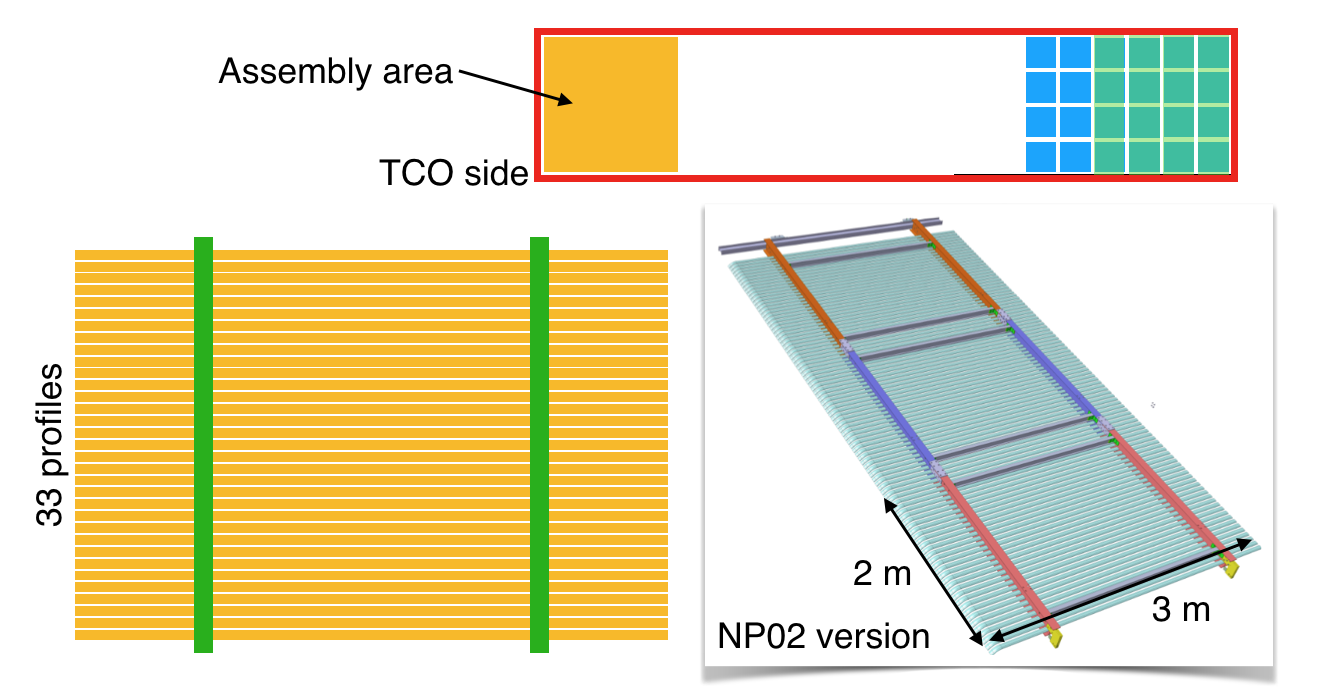
\includegraphics[width=1.\textwidth]{hv-assembly-area.png}
\end{dunefigure}

\begin{dunefigure}[]{fig:}
{.}
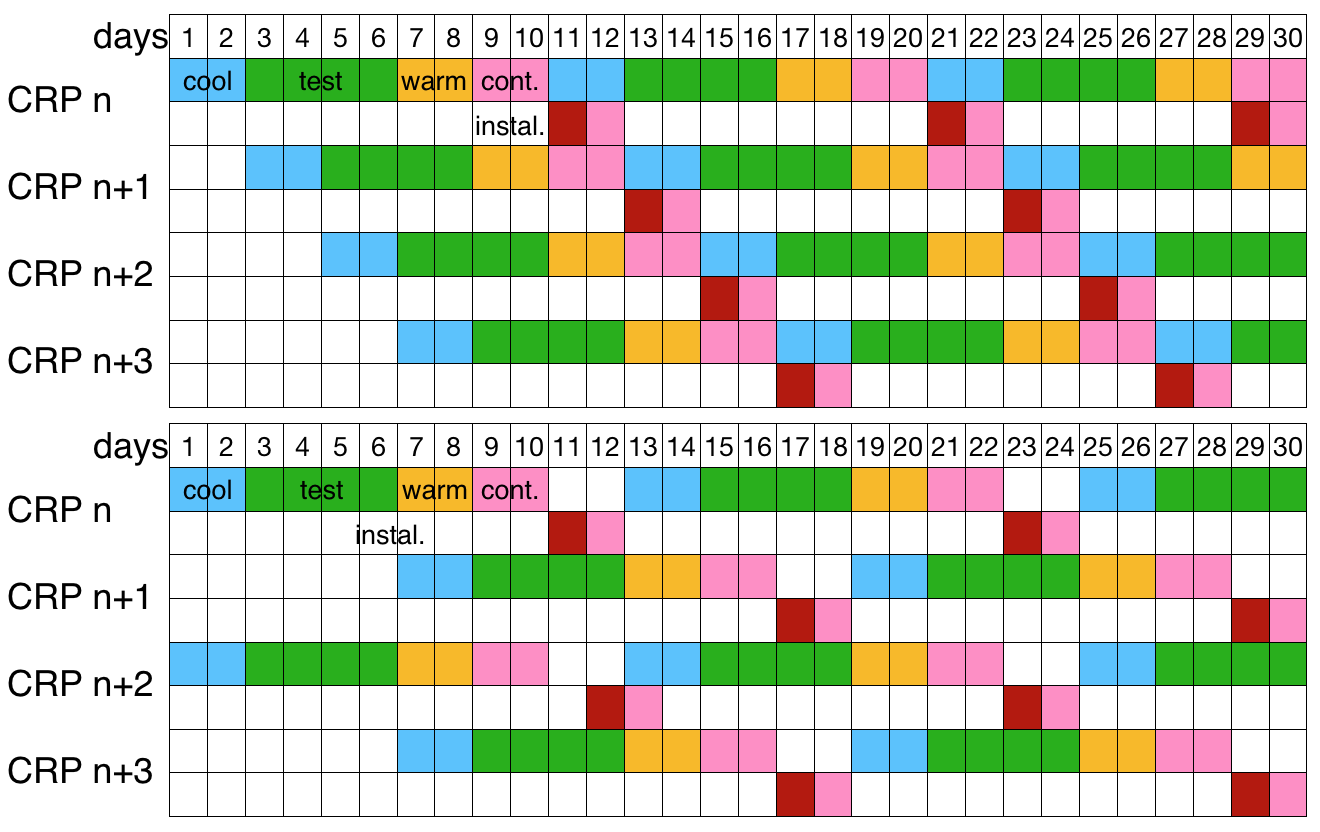
\includegraphics[width=1.\textwidth]{crp-testing-schedule.png}
\end{dunefigure}

\subsection{Charge readout plane installation}
\subsection{High voltage system installation}
\subsection{Light readout installation}
\subsection{Cryo-instrumentation installation}
\subsection{Electronics installation}
